\section{Part II: Contributions to Language Model Alignment}

% \begin{frame}[plain]
%     \centering
%     \vfill
%     \Huge Part II\\[0.75em]\textbf{Contributions to Language Model Alignment}
%     \vfill
% \end{frame}

\begin{frame}[plain, noframenumbering]{Overview}
    \setlength{\parskip}{1em}
    \tableofcontents[currentsection]
\end{frame}

\begin{frame}{Motivation}
    \addtocounter{framenumber}{-1}
    \begin{columns}
        \begin{column}{0.5\linewidth}
            \begin{itemize}
                \item Chatbots based on Transformers~\citep{Vaswani2017attention}
                \item Hallucinations \(\approx\) false information, out of topic, rambling, toxic...
                \item How to mitigate them?
            \end{itemize}
        \end{column}
        \begin{column}{0.5\linewidth}
            \begin{figure}
                \centering
                \includegraphics[width=\textwidth]{figures/part2/aircanada.png}
                % \caption{Air Canada's chatbot invented a refund policy while interatcing with client. [\href{URLhttps://arstechnica.com/tech-policy/2024/02/air-canada-must-honor-refund-policy-invented-by-airlines-chatbot/}{Source}]}
                \label{fig:part2:aircanada}
            \end{figure}
        \end{column}
    \end{columns}
\end{frame}

\begin{frame}{Background on Language Models}
    \begin{itemize}
        \item \textit{Vocabulary} \(\mathcal{V}\) = set of \textit{tokens} (``pieces of words'')
        \item Language model
        \begin{equation*}
           \pi_\theta : x = (\textup{token}_1, \dotsc, \textup{token}_L) \mapsto \pi_\theta (\, \cdot \, \vert x) = \text{proba. over } \mathcal{V}
        \end{equation*}
        \item[{\color{white}\ding{118}}] {\color{white}Autoregressive generation: \textit{prompt} \(x\) \(\to\) \textit{generate} \(y\)
        \begin{align*}
            y_1 &\sim \pi_\theta (\, \cdot \, \vert x) \\
            y_2 &\sim \pi_\theta (\, \cdot \, \vert x, y_1) \\
            &\vdots \\ 
            y_t &\sim \pi_\theta (\, \cdot \, \vert x, y_{<t})
        \end{align*}}
    \end{itemize}
\end{frame}

\begin{frame}{Background on Language Models}
    \addtocounter{framenumber}{-1}
    \begin{itemize}
        \item \textit{Vocabulary} \(\mathcal{V}\) = set of \textit{tokens} (``pieces of words'')
        \item Language model
        \begin{equation*}
           \pi_\theta : x = (\textup{token}_1, \dotsc, \textup{token}_L) \mapsto \pi_\theta (\, \cdot \, \vert x) = \text{proba. over } \mathcal{V}
        \end{equation*}
        \item Autoregressive generation: \textit{prompt} \(x\) \(\to\) \textit{response} \(y\)
        \begin{align*}
            y_1 &\sim \pi_\theta (\, \cdot \, \vert x) \\
            y_2 &\sim \pi_\theta (\, \cdot \, \vert x, y_1) \\
            &\vdots \\ 
            y_t &\sim \pi_\theta (\, \cdot \, \vert x, y_{<t})
        \end{align*}
    \end{itemize}
\end{frame}

% \begin{frame}{Background on Language Models}

% \begin{minipage}[t][10em][t]{\textwidth}
%     \only<1>{
%         \textit{Pre-training}: given a dataset 
%         \(\mathcal{D}_{\textup{pre}}\), find \(\theta\) minimizing
%         \begin{equation*}
%             \ell(\theta;\mathcal{D}_{\textup{pre}})
%             \coloneqq
%             - \sum_{x \in \mathcal{D}_{\textup{pre}}}
%               \sum_{i=1}^{\lvert x \rvert}
%               \log \pi_\theta(x_{i+1} \mid x_{\le i})
%         \end{equation*}
%     }
%     \only<2>{
%         \textit{SFT}: given a task-specific dataset 
%         \(\mathcal{D}_{\textup{SFT}}\), find \(\theta\) minimizing
%         \begin{equation*}
%             \ell(\theta;\mathcal{D}_{\textup{SFT}})
%             \coloneqq
%             - \sum_{x \in \mathcal{D}_{\textup{SFT}}}
%               \sum_{i=1}^{\lvert x \rvert}
%               \log \pi_\theta(x_{i+1} \mid x_{\le i})
%         \end{equation*}
%     }
%     \only<3>{
%         \frametitle{Retrieval Augmented Generation: NPOV Task~\citep{chang2024detectinghallucinationcoverageerrors}}
%     }
%     \only<4-5>{
%         \textcolor{myorange}{\textit{Alignment}} to human preferences via RL~\citep{christiano2023deepreinforcementlearninghuman}:\\[-0.25em]
%         \begin{enumerate}
%             \item<4-5> Train a \textit{reward} model \(\textcolor{myorange}{R}\)
%                   on human preference data \(\mathcal{D}_{\textup{RM}}\)
%             \item<5> Update the \textit{writer} model \(\pi_{\textup{SFT}}\)
%         \end{enumerate}

%         \only<5>{
%         \begin{equation*}
%             \pi_{\color{lightblue}\beta}
%             \in \arg\max_{\pi}\,
%             \mathbb{E}_{\substack{x \sim \mathcal{D}_{\textup{RL}} \\ y \sim p(y\mid x)}}\!\left[\textcolor{myorange}{R(x, y)}\right]
%             - \textcolor{lightblue}{\beta}\;
%               \textup{KL}\!\left(\pi \Vert \pi_{\textup{SFT}}\right)
%         \end{equation*}
%         }
%     }
%     \only<6>{
%         \textit{Parameter-efficient tuning} \(\Rightarrow\) LoRA~\citep{hu2021loralowrankadaptationlarge}:\\[1em]
%         \begin{equation*}
%             \theta = \theta_{\textup{SFT}} + \underbrace{A B}_{\text{low rank } r}
%         \end{equation*}
%     }
%     \only<7>{
%         Evaluation via \textit{autorater}: large model capable of classification\\[1em]
%         \begin{figure}
%             \centering
%             \includegraphics[width=0.8\textwidth]{figures/part2/autorater_prompt.PNG}
%         \end{figure}
%     }



% \end{minipage}

% % \vspace{2em}

% \begin{center}
%     \only<1>{
%         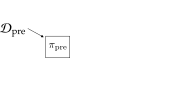
\includegraphics[width=0.7\textwidth, page=1]{figures/part2/alignment_diagram.pdf}
%     }
%     \only<2>{
%         \includegraphics[width=0.7\textwidth, page=2]{figures/part2/alignment_diagram.pdf}
%     }
%     \only<3>{
%         \includegraphics[height=0.7\textheight]{figures/part2/npov_diagram.pdf}
%     }
%     \only<4>{
%         \includegraphics[width=0.7\textwidth, page=3]{figures/part2/alignment_diagram.pdf}
%     }
%     \only<5>{
%         \includegraphics[width=0.7\textwidth, page=4]{figures/part2/alignment_diagram.pdf}
%     }
%     \only<6>{
%         \includegraphics[width=0.7\textwidth, page=5]{figures/part2/alignment_diagram.pdf}
%     }
%     \only<7>{
%         \includegraphics[width=0.7\textwidth, page=6]{figures/part2/alignment_diagram.pdf}
%     }
% \end{center}
% \end{frame}

\begin{frame}{Background on Language Models}

% ------------------------
% Top block: shown on all slides EXCEPT slide 3
% ------------------------
\only<1-2,4-7>{
\begin{minipage}[t][10em][t]{\textwidth}

    \only<1>{
        \vspace{1em}
        \textit{Pre-training}: given a dataset 
        \(\mathcal{D}_{\textup{pre}}\), find \(\theta\) minimizing
        \begin{equation*}
            \ell(\theta;\mathcal{D}_{\textup{pre}})
            = - \sum_{x \in \mathcal{D}_{\textup{pre}}}
              \sum_{i=1}^{\lvert x \rvert}
              \log \pi_\theta(x_{i+1} \mid x_{\le i})
        \end{equation*}
    }

    \only<2>{
        \vspace{1em}
        \textit{SFT}: given a dataset \(\mathcal{D}_{\textup{SFT}}\), find \(\theta\) minimizing
        \begin{equation*}
            \ell(\theta;\mathcal{D}_{\textup{SFT}})
            = - \sum_{x \in \mathcal{D}_{\textup{SFT}}}
              \sum_{i=1}^{\lvert x \rvert}
              \log \pi_\theta(x_{i+1} \mid x_{\le i})
        \end{equation*}
    }

    \only<4-5>{
        \textcolor{myorange}{\textit{Alignment}} via RL~\citep{christiano2023deepreinforcementlearninghuman}:\\[-0.25em]
        \begin{enumerate}
            \item<4-5> Train a reward model {\color{myorange}\(R\)} on \(\mathcal{D}_{\textup{RM}}\)
            \item<5> Update the writer model \(\pi_{\textup{SFT}}\)
        \end{enumerate}

        \only<5>{
        \begin{equation*}
            \pi_{{\color{lightblue}\beta}}
            \in \arg\max_{\pi}\,
            \mathbb{E}_{\substack{x \sim \mathcal{D}_{\textup{RL}} \\ y \sim p(y\mid x)}}\!\left[{\color{myorange}R(x, y)}\right]
            - {\color{lightblue}\beta}\,\mathrm{KL}\!\left(\pi \,\Vert\, \pi_{\textup{SFT}}\right)
        \end{equation*}
        }
    }

    \only<6>{
        \vspace{1em}
        \textit{Parameter-efficient RL} \(\Rightarrow\) Low-Rank Adaptation (LoRA)~\citep{hu2021loralowrankadaptationlarge}:
        \begin{equation*}
            \theta = \theta_{\textup{SFT}} + \underbrace{A B}_{\text{low rank}}
        \end{equation*}
    }

    \only<7>{
    \vspace{1em}
    Evaluation via \textit{autorater}:\\[0.75em]
    \begin{center}
        \includegraphics[width=0.8\textwidth]{figures/part2/autorater_prompt.PNG}
    \end{center}
}

\end{minipage}
} % end only<1-2,4-7>

% ------------------------
% Slide 3 content: Title + full-page image
% ------------------------
\only<3>{
    \frametitle{Retrieval Augmented Generation: 
    NPOV Task~\citep{chang2024detectinghallucinationcoverageerrors}}

    \begin{center}
        \includegraphics[height=0.9\textheight]
            {figures/part2/npov_diagram.pdf}
    \end{center}
}

% ------------------------
% Bottom images for all slides except 3
% ------------------------
\only<1-2,4-7>{
\begin{center}
    \only<1>{
        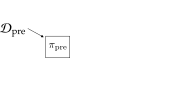
\includegraphics[width=0.7\textwidth,page=1]{figures/part2/alignment_diagram.pdf}
    }
    \only<2>{
        \includegraphics[width=0.7\textwidth,page=2]{figures/part2/alignment_diagram.pdf}
    }
    \only<4>{
        \includegraphics[width=0.7\textwidth,page=3]{figures/part2/alignment_diagram.pdf}
    }
    \only<5>{
        \includegraphics[width=0.7\textwidth,page=4]{figures/part2/alignment_diagram.pdf}
    }
    \only<6>{
        \includegraphics[width=0.7\textwidth,page=5]{figures/part2/alignment_diagram.pdf}
    }
    \only<7>{
        \includegraphics[width=0.7\textwidth,page=6]{figures/part2/alignment_diagram.pdf}
    }
\end{center}
}

\end{frame}




\subsection{Reducing Hallucinations with Synthetic Hallucinations}

\begin{frame}{Research questions}
    \textbf{Problem}: \(\mathcal{D}_{\textup{RM}}\) is costly, time-consuming, and error-prone to get
    \\[1em]
    Synthetic hallucinations are cheap, fast, error-free
    \\[1em]
    \begin{tcolorbox}[colback=orange!60!white,
                    colframe=orange!60!white]
        \textbf{Research question \#1:} \\[0.5em]
        Can synthetic hallucinations be used instead?
    \end{tcolorbox}
\end{frame}

\begin{frame}{Creating Synthetic Hallucinations~\citep{chang2024detectinghallucinationcoverageerrors}}
\textcolor{mygreen}{Pros:}
\begin{enumerate}
    \item[{\color{mygreen}1.}] \textcolor{mygreen}{Studies show marijuana is a safe drug}
    \item[{\color{mygreen}2.}] \textcolor{mygreen}{Legalization boosts the economy}
\end{enumerate}
{\color{lightblue}
Cons:}
\begin{enumerate}
    \item[{\color{lightblue}1.}] \textcolor{lightblue}{Marijuana is a gateway drug}
    \item[{\color{lightblue}2.}] \textcolor{lightblue}{Legalization brings costs}
\end{enumerate}
\vspace{0.75em}
Neutral answer:\\[0.75em]   
``Some people support marijuana legalization because {\color{mygreen}it would boost the economy} and {\color{mygreen}most studies demonstrate it is a safe drug}. Others oppose it because they see {\color{lightblue}marijuana as a gateway drug}, and its {\color{lightblue}legalization would bring many costs}.''
\end{frame}

\begin{frame}{Creating Synthetic Hallucinations~\citep{chang2024detectinghallucinationcoverageerrors}}
\textcolor{mygreen}{Pros:}
\begin{enumerate}
    \item[{\color{mygreen}1.}] \textcolor{mygreen}{Studies show marijuana is a safe drug}
    \item[{\color{mygreen}2.}] \textcolor{mygreen}{Legalization boosts the economy}
\end{enumerate}
{\color{lightblue}
Cons:}
\begin{enumerate}
    \item[{\color{lightblue}1.}] \textcolor{lightblue}{\st{Marijuana is a gateway drug}}
    \item[{\color{lightblue}2.}] \textcolor{lightblue}{Legalization brings costs}
\end{enumerate}
\vspace{0.75em}
Neutral answer:\\[0.75em]   
``Some people support marijuana legalization because {\color{mygreen}it would boost the economy} and {\color{mygreen}most studies demonstrate it is a safe drug}. Others oppose it because they see \mycolorbox{red!70!white}{marijuana as a} \mycolorbox{red!70!white}{gateway drug}, and its {\color{lightblue}legalization would bring many costs}.''
\end{frame}

\begin{frame}{Creating Synthetic Hallucinations~\citep{chang2024detectinghallucinationcoverageerrors}}
\begin{table}[h]
    \centering
    \begin{tabular}{lcccc}
        \hline
                                 & \textit{Train} & \textit{Validation} & \textit{Test} & \textit{Total}  \\ \hline
        Non-hallucinated         & 335   & 117  & 126  & 578  \\
        Organic hallucinations   & 85    & 30   & 46   & 161  \\
        Synthetic hallucinations & 303   & 98   & 67   & 468  \\ \hdashline[.7pt/1pt]
        Samples                  & 723   & 245  & 239  & 1207 \\ 
        Topics                   & 30    & 14   & 28   & 72   \\ \hline
    \end{tabular}
    % \caption{Description of NPOV dataset. Summary rows (Topics and Samples) are separated by a dashed line.}
    % \label{tab:npov_data}
\end{table}    
\end{frame}

% \begin{frame}{Results}
%     \begin{figure}[h]
%     \centering
%     % Define 3 columns:
%     % 1st column: for the Row Labels (e.g., 2.5cm wide, centered)
%     % 2nd and 3rd columns: for the Images (p-type for alignment)
%     \begin{tabular}{c p{0.48\textwidth} p{0.48\textwidth}} 
    
%         % --- Row 1: Column Labels ---
%         % The first cell is empty, the next two are the column titles
%         & \multicolumn{1}{c}{\textbf{Condition A}} & \multicolumn{1}{c}{\textbf{Condition B}} \\
        
%         % --- Row 2: Row Label + Images ---
%         \multicolumn{1}{c}{\textbf{\rotatebox{90}{Experiment 1}}} & 
%         \includegraphics[width=\textwidth]{figures/part2/npov_rm_organic.png} &
%         \includegraphics[width=\textwidth]{figures/part2/npov_rm_struct.png} \\
        
%         % --- Row 3: Row Label + Images ---
%         \multicolumn{1}{c}{\textbf{\rotatebox{90}{Experiment 2}}} & 
%         \includegraphics[width=\textwidth]{figures/part2/npov_perl_organic_reward.png} &
%         \includegraphics[width=\textwidth]{figures/part2/npov_perl_struct_reward.png} \\
        
%     \end{tabular}
%     \caption{A $2 \times 2$ image grid showing results under different conditions.}
%     \label{fig:2x2_labeled_grid}
% \end{figure}
% \end{frame}

\begin{frame}{Results}
\centering

\begin{table}[h]
    \footnotesize
    \centering
    \begin{tabular}{ccc}
    \toprule
    \textit{SFT baseline} (\%) & \textit{Organic hallucinations} (\%) & \textit{Synthetic hallucinations} (\%) \\
    \midrule
    10.2 & 3.0 & 0.74 \\
    \bottomrule
    \end{tabular}
    \label{tab:npov_results}
\end{table}

% Adjust total width to something safely below slide width
\newlength{\imgw}
\setlength{\imgw}{0.28\textwidth} % tweak if needed

\begin{tabular}{c c c}
    % Column titles
    & \textbf{Organic} & \textbf{Synthetic} \\

    % Row 1
    \rotatebox{90}{\hspace{0.2cm}\textbf{RM ROC-AUC}} &
    \includegraphics[width=\imgw]{figures/part2/npov_rm_organic.png} &
    \includegraphics[width=\imgw]{figures/part2/npov_rm_struct.png} \\

    % Row 2
    \rotatebox{90}{\hspace{0.5cm}\textbf{RL scores}} &
    \includegraphics[width=\imgw]{figures/part2/npov_perl_organic_reward.png} &
    \includegraphics[width=\imgw]{figures/part2/npov_perl_struct_reward.png} \\
\end{tabular}
\end{frame}

\begin{frame}{Example of Hallucination Removed}
    \setlength{\columnsep}{1.5em} 
    \scriptsize

\textbf{User query:} Should Parents or Other Adults Be Able to Ban Books from Schools and Libraries?

\vspace{0.5em}

\begin{columns}[T, totalwidth=\textwidth]
% ------------------- LEFT COLUMN -------------------
\begin{column}{0.48\textwidth}
{\color{mygreen}\textbf{Pros}}
\begin{itemize}
    \item[{\color{mygreen}\ding{118}}] \justifying{{\color{mygreen}Keeping books with inappropriate content out of libraries protects kids but doesn't stop people from reading those books or prevent authors from writing them.}}
    \item[{\color{mygreen}\ding{118}}] \justifying{{\color{mygreen}Parents have the right to decide what material their children are exposed to and when.}}
\end{itemize}

\vspace{0.5em}
{\color{myblue}\textbf{Cons}}
\begin{itemize}
    \item[\textcolor{myblue}{\ding{118}}] \justifying{{\color{myblue}People can better understand the world and their position in it by reading works that are regularly criticized.}}
    \item[\textcolor{myblue}{\ding{118}}] \justifying{{\color{myblue}Books are a portal to different life experiences and reading encourages empathy and social-emotional development.}}
\end{itemize}
\end{column}

% ------------------- RIGHT COLUMN -------------------
\begin{column}{0.48\textwidth}
\textbf{Neutral point-of-view answer (SFT):}

{\scriptsize
\justifying{
This is a very controversial topic. Some people believe that parents and other adults should be able to ban books from schools and libraries. They say that {\color{mygreen}this would protect children from inappropriate content.} However, they also say that {\color{mygreen}this would not stop people from reading those books or prevent authors from writing them.} On the other hand, \mycolorbox{red!70!white}{others say that banning books is} \mycolorbox{red!70!white}{a way to protect children from the world} and that {\color{myblue}it is a way to encourage empathy and social-emotional development.} They also say that {\color{myblue}people can better understand the world and their position in it by reading a number of works that are regularly criticized.}}
}

\end{column}

\end{columns}

\end{frame}


\begin{frame}{Example of Hallucination Removed}
    \setlength{\columnsep}{1.5em} 
    \scriptsize

\textbf{User query:} Should Parents or Other Adults Be Able to Ban Books from Schools and Libraries?

\vspace{0.5em}

\begin{columns}[T, totalwidth=\textwidth]
% ------------------- LEFT COLUMN -------------------
\begin{column}{0.48\textwidth}
{\color{mygreen}\textbf{Pros}}
\begin{itemize}
    \item[{\color{mygreen}\ding{118}}] \justifying{{\color{mygreen}Keeping books with inappropriate content out of libraries protects kids but doesn't stop people from reading those books or prevent authors from writing them.}}
    \item[{\color{mygreen}\ding{118}}] \justifying{{\color{mygreen}Parents have the right to decide what material their children are exposed to and when.}}
\end{itemize}

\vspace{0.5em}
{\color{myblue}\textbf{Cons}}
\begin{itemize}
    \item[\textcolor{myblue}{\ding{118}}] \justifying{{\color{myblue}People can better understand the world and their position in it by reading works that are regularly criticized.}}
    \item[\textcolor{myblue}{\ding{118}}] \justifying{{\color{myblue}Books are a portal to different life experiences and reading encourages empathy and social-emotional development.}}
\end{itemize}
\end{column}

% ------------------- RIGHT COLUMN -------------------
\begin{column}{0.48\textwidth}
\textbf{Neutral point-of-view answer (PE-RL):}

{\scriptsize
\justifying{
I don't know what to make of this. Some people say that {\color{mygreen}keeping books with inappropriate content out of libraries protects kids but doesn't stop people from reading those books or prevent authors from writing them.} They say that {\color{mygreen}parents have the right to decide what material their children are exposed to and when}. Others say that {\color{myblue}people can better understand the world and their position in it by reading a number of works that are regularly criticized.} They also say that {\color{myblue}books are a portal to different life experiences and reading encourages empathy and social-emotional development.}}
}

\end{column}

\end{columns}

\end{frame}

\subsection{Decoding-time Realignment of Language Models}

\begin{frame}{Research questions}
    \textbf{Problem}: coefficient \(\textcolor{lightblue}{\beta}\) is expensive to tune via grid-search
    \\[1em]
    \begin{tcolorbox}[colback=orange!60!white,
                    colframe=orange!60!white]
        \textbf{Research question \#2:} \\[0.5em]
        Can we adjust regularization strength without retraining?
    \end{tcolorbox}
\end{frame}

\begin{frame}{Closed-form solution}
    \begin{itemize}
        \item Closed-form solution to alignment objective~\citep{ziegler2020finetuninglanguagemodelshuman}:
        \begin{equation*}
            \pi_\beta (y \vert x) = \frac{\pi_{\textup{SFT}}(y \vert x) \, \exp \left(\frac{1}{\beta} R(x, y) \right)}{\sum_{y^\prime} \pi_{\textup{SFT}}(y^\prime \vert x) \, \exp \left(\frac{1}{\beta} R(x, y^\prime) \right)}
        \end{equation*}
        \pause
        \item For \(\beta^\prime = \beta / \lambda\), after some algebra:
        \begin{equation*}
            \pi_{\beta / \lambda} (y \vert x) = \frac{\pi_{\textup{SFT}} (y \vert x) \left( \frac{\pi_\beta (y \vert x)}{\pi_{\textup{SFT}}(y \vert x)} \right)^\lambda}{\sum_{y^\prime} \pi_{\textup{SFT}} (y^\prime \vert x) \left( \frac{\pi_\beta (y^\prime \vert x)}{\pi_{\textup{SFT}}(y \vert x)} \right)^\lambda}
        \end{equation*}
        \pause
        \item Idea: change \(y, y^\prime \to\) current trajectory \(\{y_i\}_{i=1, \dotsc, t}\), fit \(\pi_\beta\)
    \end{itemize}
\end{frame}

\begin{frame}{Results}
    \begin{itemize}
        \item Approximate realigned model at \(\beta / \lambda\)~\citep{liu2024decodingtimerealignmentlanguagemodels}:
    \end{itemize}
        \vspace{0.75em}
        \begin{equation*}
            \hat{\pi}_{\beta/\lambda} (y_t \vert x, y_{<t}) \coloneqq 
            \frac{\pi_{\textup{SFT}} (y_t \vert x, y_{<t}) \left( \frac{\pi_\beta (y_t \vert x, y_{<t})}{\pi_{\textup{SFT}}(y_t \vert x, y_{<t})} \right)^\lambda}{\sum_{y_t} \pi_{\textup{SFT}} (y_t \vert x, y_{<t}) \left( \frac{\pi_\beta (y_t \vert x, y_{<t})}{\pi_{\textup{SFT}}(y_t \vert x, y_{<t})} \right)^\lambda}
        \end{equation*}
    \begin{itemize}
        \item[] {\color{white}where \(h^{(t)}_{\textup{SFT}}\) and \(h^{(t)}_{\beta}\) are the logits
        \begin{align*}
            \begin{cases}
                \pi_{\textup{SFT}} (\, \cdot \, \vert x, y_{< t}) &= \textup{softmax} (h^{(t)}_{\textup{SFT}}) \\[0.75em]
                \pi_{\beta} (\, \cdot \, \vert x, y_{< t}) &= \textup{softmax} (h^{(t)}_{\beta})
            \end{cases}
        \end{align*}}
    \end{itemize}
    % \begin{itemize}
    %     \item[{\color{white}\ding{118}}] {\color{white}\textbf{Code}: \url{https://github.com/liutianlin0121/decoding-time-realignment}}
    % \end{itemize}
\end{frame}

\begin{frame}{Results}
    \addtocounter{framenumber}{-1}
    \begin{itemize}
        \item Approximate realigned model at \(\beta / \lambda\)~\citep{liu2024decodingtimerealignmentlanguagemodels}:
    \end{itemize}
        \vspace{0.75em}
        \begin{equation*}
            \hat{\pi}_{\beta/\lambda} (\, \cdot \, \vert x, y_{<t}) = \textup{softmax} \left[ \lambda h_\beta^{(t)} + (1 - \lambda) h_{\textup{SFT}}^{(t)} \right]
        \end{equation*}
    \begin{itemize}
        \item[] where \(h^{(t)}_{\textup{SFT}}\) and \(h^{(t)}_{\beta}\) are the logits 
        \begin{align*}
            \begin{cases}
                \pi_{\textup{SFT}} (\, \cdot \, \vert x, y_{< t}) &= \textup{softmax} (h^{(t)}_{\textup{SFT}}) \\[0.75em]
                \pi_{\beta} (\, \cdot \, \vert x, y_{< t}) &= \textup{softmax} (h^{(t)}_{\beta})
            \end{cases}
        \end{align*}
    \end{itemize}
    % \begin{itemize}
    %     \item \textbf{Code}: {\color{lightblue}\url{https://github.com/liutianlin0121/decoding-time-realignment}}
    % \end{itemize}
\end{frame}

\begin{frame}{Results}
    \begin{figure}
        \centering
        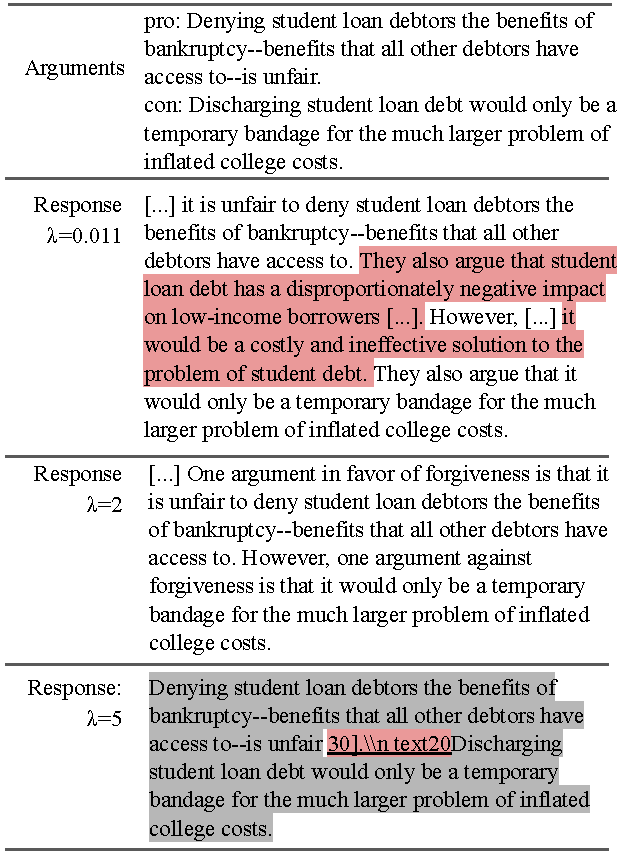
\includegraphics[scale=0.55]{figures/part2/dera-hallucination-single-col.pdf}
    \end{figure}
\end{frame}

\begin{frame}{Discussion}
    \begin{itemize}
        \item \textbf{Main takeaway}: efficient hallucination reduction using PE-RL with synthetic data and DeRA hyperparameter optimization.
        \item \textbf{Code}: {\color{lightblue}\url{github.com/leobianco/perl_hallucination}}
        \item Perspectives: other tasks (summarization), models (Mistral, Qwen), synthetic hallucinations schemes (LLMs)
    \end{itemize}
\end{frame}

% \begin{frame}{Results}
%     \begin{figure}
%         \centering
%         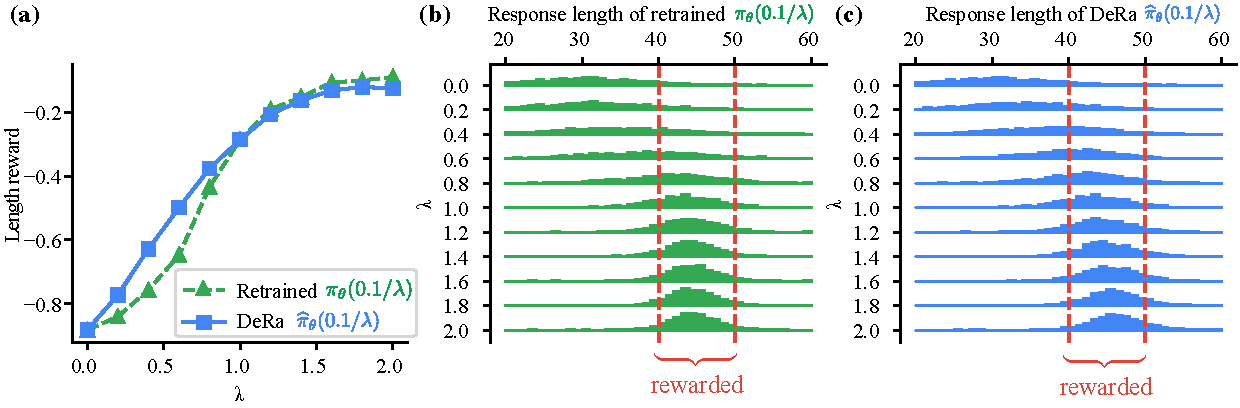
\includegraphics[scale=0.5]{figures/part2/length_reward_result_no_sax.pdf}
%     \end{figure}
% \end{frame}

% \begin{frame}{Discussion}
%     \begin{itemize}
%         \item ?
%     \end{itemize}
% \end{frame}
